\documentclass{article}


\usepackage{xcolor} 
\usepackage{enumerate}

\usepackage{graphicx}
%\pagecolor{black!100}
%\color{gray!100}



\begin{document}
	\section*{Concordia University}
	\hfill \\\hfill \\\hfill
	{\centering{
			\section*{System Hardware - comp228}
			\textbf{Professor}: Kerly Titus
			\textbf{Section}: U

		}}

	\hfill \\
	\hfill \\
	\hfill \\\hfill \\
	\hfill \\\hfill \\
	\noindent \textbf{Student id}: 6517722\\
	\textbf{Student name}: Hani Sayegh\\
	\textbf{Data submitted}: 12/02/2014\\
	\hfill \\
	\hfill \\\hfill \\
	\hfill \\\hfill \\
	\textbf{Theory assignment} \# 4\\
	\textbf{Programming assignment} \# 3\\
	\hfill \\
	\hfill \\\hfill \\
	\textbf{Grade}: \verb|    /100|
	\hfill \\\hfill \\
	\hfill \\\hfill \\
	\hfill \\\hfill \\
	\hfill \\\hfill \\
	\hfill \\\hfill \\
	\hfill \\\hfill \\
	\hfill \\\hfill \\
	\hfill \\\hfill \\
	\textbf{Department of Computer Science and Software Engineering, Fall 2014}

	1)\\
	a)
	\begin{enumerate}[i]
		\item Load 100. AC = 200, PC = 201 
		\item Subt 100. AC = -100, PC = 201
		\item AddI 100. AC = 400, PC = 201
		\item Jns 100. AC = 101,  M[100] = 201, M[200] = 300, PC = 101.
	\end{enumerate}
	b)
\\
Load 200\\
\begin{tabular}{l*{6}{c}r}
Step              & RTN & PC & IR & MAR & MBR  & AC \\
\hline
Initial Values    &     & 100 &  &  &  &  1000\\
Fetch            & MAR \verb|<-| PC & 100 &  & 100 &   &  1000\\
                 & IR \verb|<-| M[MAR] & 100 & 1200 & 100 &   & 1000 \\
                & PC \verb|<-| PC + 1 & 101 & 1200 & 100 &   &  1000\\
Decode     &  MAR \verb|<-| IR[11-0] & 101 & 1200 & 200 &   &  1000\\
     &  (Decode IR[15-12]) & 101 & 1200 & 200 &   &  1000\\
Get operand &    MBR \verb|<-| M[MAR] & 101 & 1200 & 200 &  FFFF & 1000 \\
Execute &    AC \verb|<-| MBR & 101 & 1200 & 200 &  FFFF &  FFFF\\
\end{tabular}
\\
\\
\\
Add 200
\\
\\
\begin{tabular}{l*{6}{c}r}
Step              & RTN & PC & IR & MAR & MBR  & AC \\
\hline
Initial Values    &     &  101 & 1200 & 200 &  FFFF &  FFFF\\
Fetch            & MAR \verb|<-| PC &  101 & 1200 & 101 &  FFFF &  FFFF\\
                 & IR \verb|<-| M[MAR] &  101 & 3200 & 101 &  FFFF &  FFFF\\
                & PC \verb|<-| PC + 1 & 102 & 3200 & 101 &  FFFF &  FFFF\\
Decode     &  MAR \verb|<-| IR[11-0] & 102 & 3200 & 200 &  FFFF &  FFFF\\
     &  (Decode IR[15-12]) &  102 & 3200 & 200 &  FFFF &  FFFF\\
Get operand &    MBR \verb|<-| M[MAR] & 102 & 3200 & 200 &  FFFF &  FFFF\\
Execute &    AC \verb|<-|AC + MBR & 102 & 3200 & 200 &  FFFF &  FFFE\\
\end{tabular}
\\
\\
\\
jns 300
\\
\\
\begin{tabular}{l*{6}{c}r}
Step              & RTN & PC & IR & MAR & MBR  & AC \\
\hline
Initial Values    &     &  102 & 3200 & 200 &  FFFF &  FFFE\\
Fetch            & MAR \verb|<-| PC &  102 & 3200 & 102 &  FFFF &  FFFE\\
                 & IR \verb|<-| M[MAR] &  102 & 0300 & 102 &  FFFF &  FFFE\\
                & PC \verb|<-| PC + 1 & 103 & 0300 & 102 &  FFFF &  FFFE\\
Decode     &  MAR \verb|<-| IR[11-0] & 103 & 0300 & 300 &  FFFF &  FFFE\\
     &  (Decode IR[15-12]) &  103 & 0300 & 300 &  FFFF &  FFFE\\
Get operand &    MBR \verb|<-|  PC& 103 & 0300 & 300 &  103 &  FFFE\\
&    M[MAR]\verb|<-|  MBR& 103 & 0300 & 300 &  103 &  FFFE\\
&  MBR\verb|<-|  300& 103 & 0300 & 300 &  300 &  FFFE\\
&  AC\verb|<-|  1& 103 & 0300 & 300 &  103 &  1\\
Execute &    AC \verb|<-|AC + MBR & 103 & 0300 & 300 &  103 &  104\\
 &    PC \verb|<-|AC & 104 & 0300 & 300 &  103 &  104\\
\end{tabular}
\\
c)
\begin{enumerate}[i]
	\item  To me it conveys that the label Data is a representaion of address 00B and addresses 002 and 003 contain references (data values) of 00B.
		
	\item 00B, 00D, 00C, 000, 00A.
	\item 200B, 8400, 000A, 004 \& 006.
	\item Instruction at S will be executed 10 times. We would have 10 inputs, but since we do not know what is the input we will call them a, b, c, d, e, f, g, h, i, j. So at Data we would have:\\
		j - (i - ( h - ( g - ( f - ( e - ( d - ( c - ( b - (a - 48)))))))))
\end{enumerate}
2.
a)
\begin{enumerate}
	\item Minimum number of k required is 7, because we have 100 opcodes and the smallest multiple of 2 greater than or equal to 100 is $2^7$.
	\item Minimum value of n is 27, because we have $2^7$ by $2^{20}$ words, which is $2^{27}$.
	\item Maximum opcodes that could be used is 128.

\end{enumerate}
b)
\begin{enumerate}
	\item  Minimum n would be 33 bits, because we need at least 5 bytes to represent 27 + 7 bits as a word to the closest number of integer bytes.
	\item Largest memory would be $2^{32} =4294967296$.
\end{enumerate}
3.
a)
\begin{enumerate}
	\item Total number of clock cycles is 11, since we need 4 clock cycles to load the data into AC, then we can Store it whch will take another 4 clock cycles after the AddI's are done, however since this is a pipelined processor both AddI can happen simultaneously while loading.
\end{enumerate}
b)

\begin{enumerate}
	\item We have to use the following formula, $S = \frac{nt_n}{(k + n - 1)t_p}$.
	\item k is 4 since we have 4 stages.
	\item n is 4 since we have 4 instructions.
	\item Plugging in we have: $S = \frac{16}{7}$.
\end{enumerate}
c)
\begin{enumerate}
	\item Resource conflicts.
		\begin{enumerate}
			\item Instructions in the pipeline may require simultaneous access to shared resources such as memory, register, bus, etc.
		\end{enumerate}
	\item  Data dependencies. 
		\begin{enumerate}
			\item The following instructions that are in the pipeline may need data from the current instruction.
		\end{enumerate}
	\item Conditional branch dependencies. 
		\begin{enumerate}
			\item A branch instruction may alter the flow of execution and the instructions following the branch may not execute.
		\end{enumerate}
\end{enumerate}
4.\\
a)
\begin{enumerate}
	\item  
		\begin{verbatim}
			MAR <- FFF    /FFF
			MBR <- M[MAR] / F01
			AC <- -1      / -1
			AC <- AC + MBR // F00
			M[MAR] <- AC /FFF has F00 now
			MAR <- MBR /F01
			MBR <- M[MAR] /1234
			MAR <- AC /F00
			M[MAR] <- MBR /F00 has 1234 now
		\end{verbatim}
	\item Yes it can:
		\begin{verbatim}
			LoadI stackPointer  /1234 in AC
			
			Store valueToDuplicate /1234 in valueToDuplicate
			Load negativeOne / -1 in AC
			Add stackPointer /F00 in AC.

			Store stackPointer /F00 in stackPointer.
			load valueToDuplicate / 1234 in AC
			StoreI stackPointer /Address F00 now contains 1234.

			stackPointer, F01 HEX /Assume stackPointer at FFF
			negativeOne, -1 DEC
			valueToDuplicate, 0 DEC
		\end{verbatim}
\end{enumerate}

5.\\
a)
\begin{enumerate}
	\item  The cache has a total size of $2^9 \times 2^{10} = 2^ {19}$bytes.
		\item We know that each block (line) has max of 8 bytes. 
		\item So we have $\frac{2^{19}}{2^3} = 2^{16}$ blocks in cache.
		\item Main memory has $\frac{2^9 \times 2^{20}}{2^2} = 
			2^{27}	words.$
		\item  So memory has $\frac{2^{27}}{2} = 2^{26}$ blocks.
		\item FOR DIRECT WE HAVE: 1 for word. 16 for block in cache. 10 for tag.
		\item FOR ASSOCIATIVE: it is 1 for word and 26 for tag.
		\item FOR TWO WAY SET ASSOCIATIVE: we have 1 for word, 11 for tag and 15 for set.
	\end{enumerate}
	b)\\
	\begin{enumerate}[i]
		\item Progrmmed I/O should be used for transfer of large data sets.
		\item Interrupt driven I/O for transfer of few bytes.
		\item DMA for transfer of a few bytes within a given time limit.
	\end{enumerate}
6.\\
\begin{verbatim}
WHILE,     INPUT         /INPUT A VALUE IN ASCII
           SUBT BORDER   /SUBTRACT 48 TO CONVERT INTO DECIMAL
           SKIPCOND 000  /IF NEGATIVE HALT IMMEDIATELY, THIS IS NOT A DIGIT
           JUMP ELSE
           JUMP ENDLOOP
ELSE,      SKIPCOND 400 /SKIP IF INPUT IS 0
           JUMP ISDIGIT
           JUMP INCREMENT
ISDIGIT,   SUBT MAX /SUBTRACT 9 TO SEE IF IT IS DIGIT
           SKIPCOND 800 /SKIP IF MORE THAN 0,
	                       / THIS MEANS IT IS NOT A DIGIT SO TERMINATE
           JUMP WHILE   /WHILE WE HAVE INPUT
           JUMP ENDLOOP

INCREMENT, LOAD COUNT
           ADD FOUND  /INCREMENT NUMBER OF 0'S BY 1
           STORE COUNT
           JUMP WHILE /WHILE WE HAVE INPUT

ENDLOOP, LOAD COUNT
         OUTPUT
         HALT


FOUND,  DEC 1 /ADD 1 EVERYTIME WE FIND A 0
BORDER, DEC 48 /SUBTRACT48 TO CONVERT FROM ASCII TO DECIMAL
MAX,    DEC 9 /IF WE SUBTRACT 9 FROM DECIMAL AND IT 
              /IS GRETER THAN 0 THEN IT IS NOT A DIGIT
COUNT, DEC 0 /VARIABLE THAT CONTAINS NUMBER OF 0'S
\end{verbatim}
	\begin{figure}[ht!]
\centering
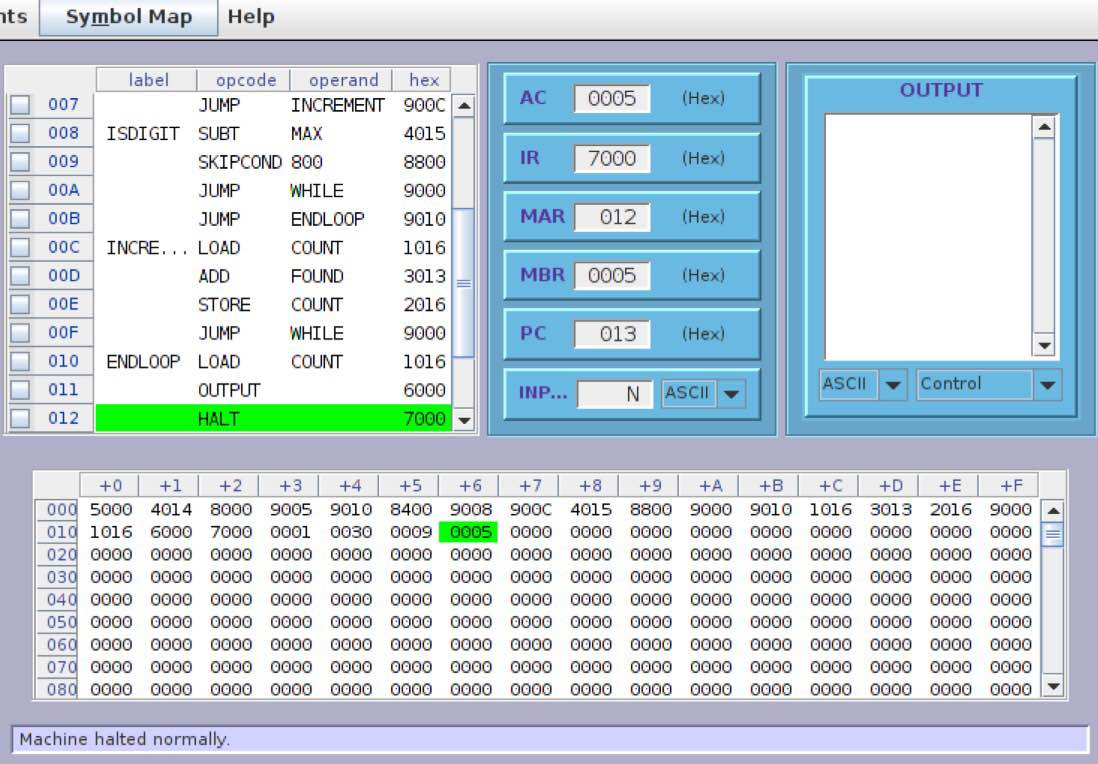
\includegraphics[width=120mm]{sim.jpg}
\caption{A simulation with five 0's occurring and halted by ASCII key N \label{overflow}}
\end{figure}
	
\begin{figure}[ht!]
\centering
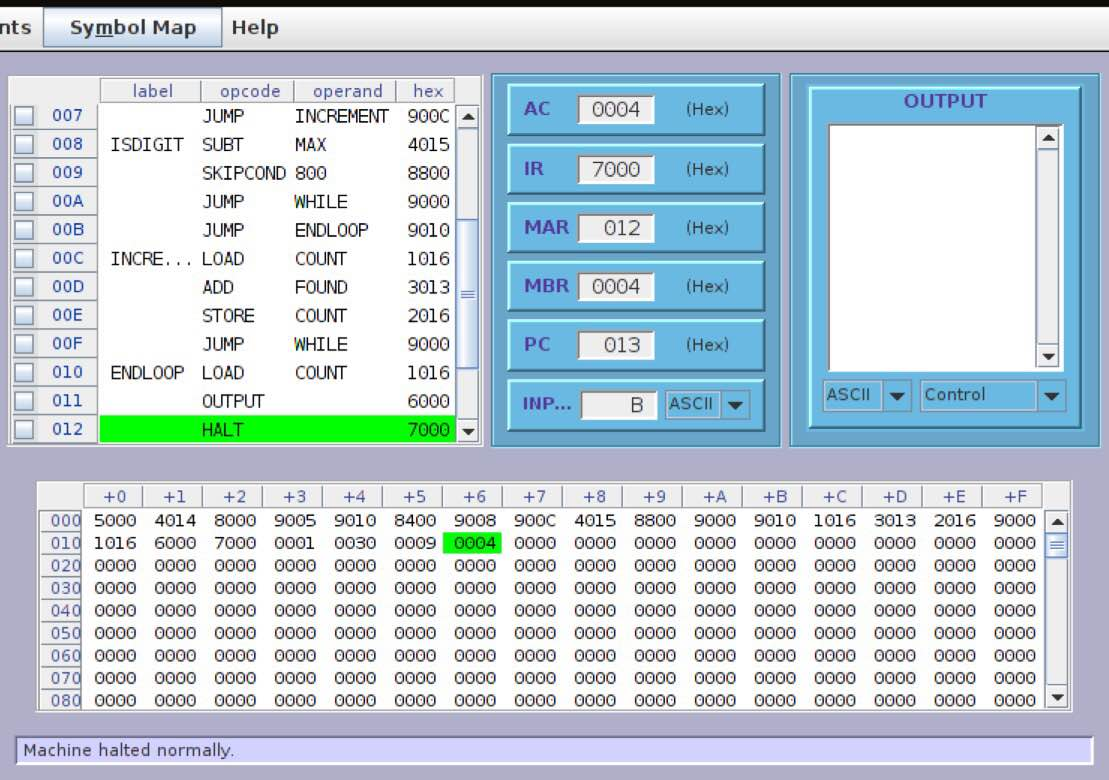
\includegraphics[width=120mm]{sim2.jpg}
\caption{A simulation with four 0's occurring and halted by ASCII key B \label{overflow}}
\end{figure}














\end{document}
